\documentclass[12 pt]{article}
\usepackage[utf8]{inputenc}
\usepackage{fancyvrb}
\usepackage{titlesec}
\usepackage{lscape}
\usepackage[table,xcdraw]{xcolor}

\usepackage{tikz}
\usetikzlibrary{shapes.geometric, arrows}
\tikzstyle{beginend} = [rectangle, rounded corners, minimum width=3cm, minimum height=1cm,text centered, draw=black, fill=white!30]
\tikzstyle{process} = [rectangle, minimum width=3cm, minimum height=1cm, text centered, draw=black, fill=orange!30]
\tikzstyle{decision} = [diamond, minimum width=3cm, minimum height=1cm, text centered, draw=black, fill=green!30]
\tikzstyle{arrow} = [thick,->,>=stealth]

\newcolumntype{L}{>{\centering\arraybackslash}m{5cm}}

\setcounter{secnumdepth}{0}
\makeatletter
\renewcommand{\l@section}{\@dottedtocline{1}{2.5em}{2.3em}}
\makeatother
\setlength\parindent{24pt}

\title{Final Project Proposal}
\author{Paul Plew}
\date{April 2, 2021}

\begin{document}

\maketitle

\section*{Summary}
\hspace*{\parindent} For the final project I have decided to make a program that generates mazes procedurally. There will be two different ways to use the program. The first being a visual demonstration of a maze generating algorithm where the user can choose the number of cells on the width and the height. The program will then generate a maze using one of a few algorithms. Right now I have decided to demonstrate maze generation using the \verb|depth-first|, and the \verb|Kruskal's| algorithms. The second way the user can use this program is to create printable mazes that can be solved by hand. My main goal in this project is to make the program as memory and CPU efficient as possible, so it can be run on potato browsers. \\
\hspace*{\parindent}  I am also planning to add a maze solving mode that implements an AI that can solve mazes. Like the generation of Mazes I would like to demonstrate two different algorighms. One such algorithm is the \verb|Wall follower| algorithm that will stick on either the right or left wall and turn when that wall turns. A second algorim candidate is \verb|Trémaux's algorithm| which has a few rules. In this algorithm the paths are marked once each time they are passed, and if the path has been marked twice that is not a solution and the solver will move on.
\newpage
\section{Plans}
\subsection{Plan 1: Murphy's Law Plan}
\hspace*{\parindent} April 9: Create Canvas and Start page with buttons \\
\hspace*{\parindent} April 16: Start depth-first maze generator \\
\hspace*{\parindent} April 23: Finish depth-first maze generator \\
\hspace*{\parindent} April 28: Start Kruskal's maze generator \\
\hspace*{\parindent} April 30: Finish Kruskal's maze generator 
\subsection{Plan 2: Blue Sky Plan}
\hspace*{\parindent} April 9: Finish Start page and depth-first generator\\
\hspace*{\parindent} April 16: Finish Kruskal's maze generator\\
\hspace*{\parindent} April 23: Make Printable Maze page \& Playable Maze page\\
\hspace*{\parindent} April 25: Finish Maze solving AI\\
\hspace*{\parindent} April 30: Finalize, fix bugs, Add color selection and size selection\\

\newpage
\section{Software Specification}
\subsection{Technical Information}
\hspace{\parindent} This program will use a cell class to contain a cell with walls. The walls will be removed depending on how the algorithm progresses through them. Each maze will be an array of these cells behind the scenes and as the mazes are generated the array of cells will be updated, and iterated over multiple times. \\
\hspace*{\parindent} The program will have two different `modes' where the user can either watch mazes generate over and over until they find one they want to print, or a mode where the user can solve an algorithmically generated maze (either in the application itself or printed out and solve it by hand). \\
\hspace*{\parindent} The javascript will be written using the \verb|p5.js| libraries and will contain two top classes. The first class will represent cells and the second will represents the world. The world class will be extended by multiple subclasses, each representing a state of the world. These classes will be named like: \verb|start| \verb|generate|, \verb|play|, and \verb|print|. The draw function will then ask the world object what the current state is and will show the appropriate state
\subsection{User Story Pseudo Code}
\verb|user|:
\hfill\begin{minipage}{\dimexpr\textwidth-1cm}
	``As someone who LOVES mazes I want to learn more about how computers generate mazes and I want to play some at the same time! Oh how I wish I had a way to do that. Every day I go without playing mazes and learning I get more grumpy and my family is starting to complain :(''
\end{minipage}\\ \\

\verb|Enter Maze Generator| \\ \\ \\
\verb|user|:
\hfill\begin{minipage}{\dimexpr\textwidth-1cm}
	``OMG!! All of my problems are solved and I am no longer grumpy I love seeing these maze generation algorithms and the mazes they generate are so fun to solve. I can even print them out and my kids can solve them. This is truly fun for the whole family.''
\end{minipage}
\subsection{Flow Chart Pseudo Code}
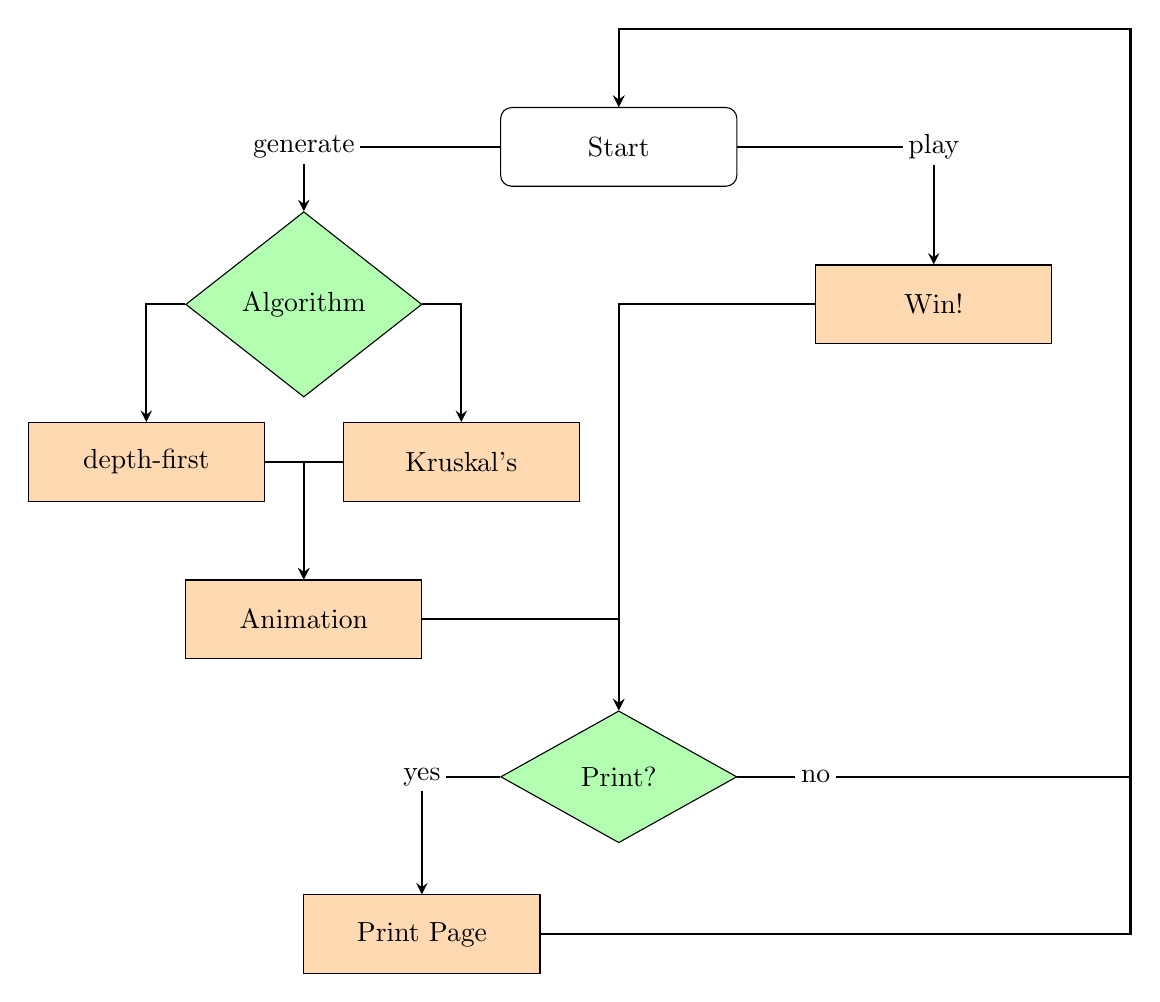
\begin{tikzpicture}[node distance=2cm]
	\node (start) [beginend] {Start};
	\node (select) [decision, below of=start, xshift=-4cm] {Algorithm};
	\node (win) [process, below of=start, xshift=4cm] {Win!};d
	\node (depth-first) [process, below of=select, xshift=-2cm] {depth-first};
	\node (kruskal) [process, below of=select, xshift=2cm] {Kruskal's};
	\node (animate) [process, below of=depth-first, xshift=2cm] {Animation};
	\node (print) [decision, below of=animate, xshift=4cm] {Print?};
	\node (ppage) [process, below of=print, xshift=-2.5cm] {Print Page};

	\draw [arrow] (start) -| node[fill=white,inner sep=2pt] {generate} (select);
	\draw [arrow] (select) -| (depth-first);
	\draw [arrow] (select) -| (kruskal);
	\draw [arrow] (depth-first) -| (animate);
	\draw [arrow] (kruskal) -| (animate);
	\draw [arrow] (animate) -| (print);
	\draw [arrow] (print) -| node[fill=white,inner sep=2pt] {yes}(ppage);
	% \draw [arrow] (print) |- (start);
	\draw [arrow] (start) -| node[pos=0.4,fill=white,inner sep=2pt, xshift=0.5cm] {play} (win);
	\draw [arrow] (win) -| (print);
	\draw [arrow] (print) -| node[fill=white,inner sep=2pt, xshift=-4cm] {no}+(right:6.5cm) |- +(up:9.5cm) -- (start);
	\draw [arrow] (ppage) -| +(right:9cm) |- (up:1.5cm) -- (start);
\end{tikzpicture}

\newpage
\pagenumbering{gobble}
\begin{landscape}
\centering 
	\begin{table}[h]
	\centering
		\begin{tabular}{|l|L|L|L|}
			\hline
			\cellcolor[HTML]{C0C0C0} Component &
			\cellcolor[HTML]{C0C0C0} Excellent (9-10) &
			\cellcolor[HTML]{C0C0C0} Competent (4-8) &
			\cellcolor[HTML]{C0C0C0} Not yet Competent (0-3)\\ 
			\hline

			\cellcolor[HTML]{EFEFEF}Objectives &
			All major and minor objectives are met including those that are not required. &
			All major and minor objectives are met, but not exceeded. &
		    Major and/or minor objectives are not met.\\
			\hline
			\cellcolor[HTML]{EFEFEF}Design &
			Application looks clean and polished. The student obviously put a lot of time and effort into how it is presented. &
			The application is clean, but not as polished as it could be. The student put some time and effort into how it is presented. &
			There are obvious visual elements missing the student had trouble creating and placing different elements. \\ 
			\hline
			\cellcolor[HTML]{EFEFEF}Programming & 
			Student shows advanced knowledge of programming principles such as: Scope, Classes, Inheritance, etc. &
			Student shows knowledge of programming principles but misses a few. &
		 	Student shows lack of understanding regarding some programming principles. \\
			\hline
			\cellcolor[HTML]{EFEFEF}Comments/Readability & 
			Student put effort into making their code readable and added comments for readers to better understand what is occurring. &
			Student put some effort into comments and code readability, but there could be some improvement &
			Student missed out on many opportunities to explain aspects of the application. \\
			\hline
		\end{tabular}
	\end{table}
\end{landscape}

\end{document}
